\documentclass{article}
\usepackage[utf8]{inputenc}
\usepackage{amsmath}
\usepackage{graphicx}
\title{Homework 3 Solution}
\author{Qazi Umer Jamil }
% 34 MTS B%
%EE379 - Linear Control Systems (LCS)%
\date{January 15, 2016}

\begin{document}

\maketitle

\section{Solution of Problem 50}

\subsection{Given Problem}
The block diagram of system is

\begin{figure}[h]
  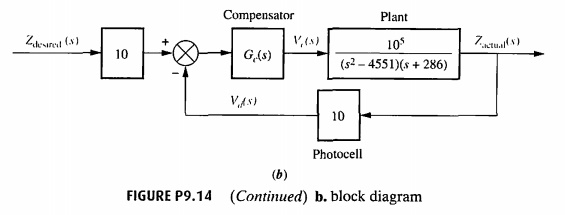
\includegraphics[width=\linewidth]{block_diagram.jpg}
  \caption{Block Diagram}
  \label{fig:boat1}
\end{figure}

Pushing 10 to the right of the summing junction, we have

\[ G(s)=\frac{10^6}{(s^2 - 4551)(s+286)} \]

The above transfer function has a pole at +67.41. This means that the system is stable since one of its pole is in right half plane.
\\
The Root Locus of G(s) is shown in Figure 2.
\begin{figure}[h]
  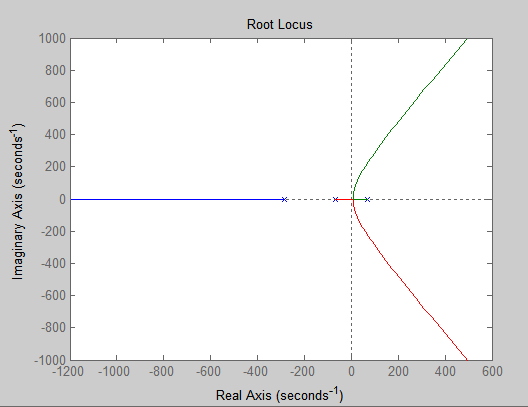
\includegraphics[width=\linewidth]{fig_1.PNG}
  \caption{Root Locus of G(s)}
  \label{fig:boat1}
\end{figure}


\subsection{PD Compensator Design}
Given:
\\
\[ T_s = 0.1 sec \]
\\
and
\\
\[ OS = 0.01\]
\\
so  \[\zeta = 0.826 \] 
\\
As
\[ \zeta = cos{\theta} \] 
\\
So
\[ \theta = 34.30 \]
The real part of the dominant pole can be found as
\[ b = \sigma \tan{\theta} \]
\[ b = 40 \tan{34.30} \]
\[ b = 27.29 \]
So, the dominant poles are located at -40+27.29j and -40-27.29j
The angle contribution of each pole can be calculates as follow. (As shown in Figure 3)
\begin{figure}[h]
  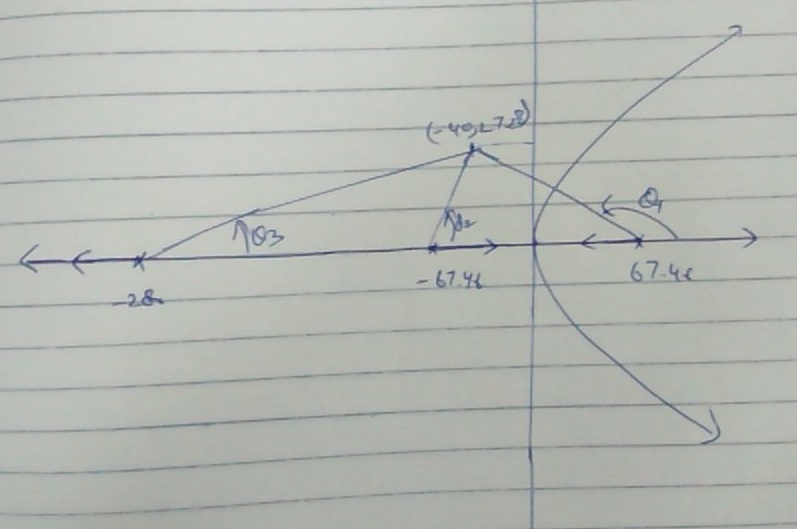
\includegraphics[width=\linewidth]{dom_pole.jpg}
  \caption{Angle contribution from each pole}
  \label{fig:boat1}
\end{figure}
\[\theta_1 = 180 - \arctan{\frac{27.28}{(40+67.46)}} \]
\[\theta_1 = 165.75\]

\[\theta_2 = \arctan{\frac{27.28}{(-40+67.46)}} \]
\[\theta_2 = 44.52\]

\[\theta_3 = \arctan{\frac{27.28}{(-40+286)}} \]
\[\theta_3 = 6.32\]
\\
So, angel contribution needed from the compensator's zero is 165.75 + 44.52 + 6.32 - 180 = 36.59

\begin{figure}[h]
  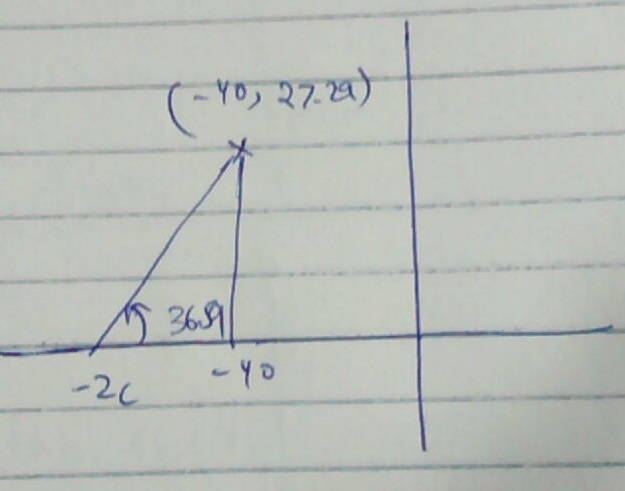
\includegraphics[width=\linewidth]{zero_c.jpg}
  \caption{Angle contribution from Compensator Zero}
  \label{fig:boat1}
\end{figure}

\[\tan{36.59} = \frac{27.28}{(z_c+286)} \]
The above equation give us 
\[ z_c = 76.75 \]
So the compensator zero is located at -76.75.
\\
The Gain K for the compensated system can be calculated as follows:
\[ K = \frac{(\sqrt{27.28^2 + (40+67.46)^2})(\sqrt{27.28^2 + (40-67.46)^2})(\sqrt{27.28^2 + (280-40)^2})}{(\sqrt{27.28^2 + (76.56-40)^2})} \]
\[ K= 22745.27\]
The root locus of compensated system is shown in Figure 5(on the next page).
\begin{figure}[h]
  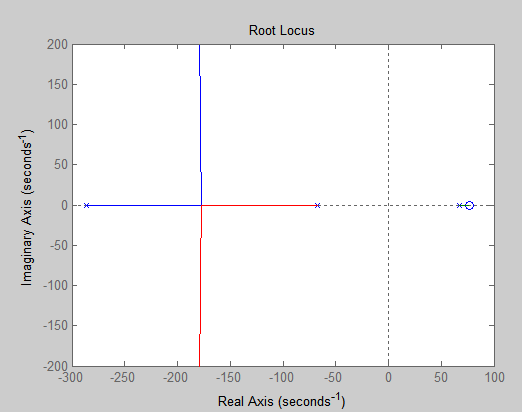
\includegraphics[width=\linewidth]{fig2.PNG}
  \caption{Root locus of compensated system}
  \label{fig:boat1}
\end{figure}

\subsection{PI Compensator Design}
To minimize the steady state error without effecting the transient response, we can use PI compensator given as follows:
\[ G(s) = \frac{s+0.1}{s} \]
The root locus of resulted compensated system is shown in Figure 6.
\begin{figure}[h]
  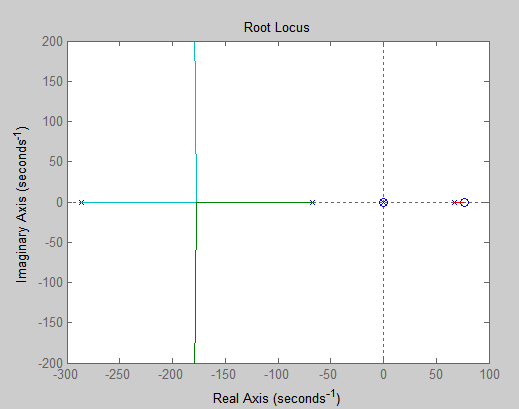
\includegraphics[width=\linewidth]{fig3.PNG}
  \caption{Root locus of compensated system (PI)}
  \label{fig:boat1}
\end{figure}

\subsection{Simulations}
\subsubsection{Simulation after adding a zero}
The simulation is shown in Figure 6 on the next page.a\begin{figure}[h]
  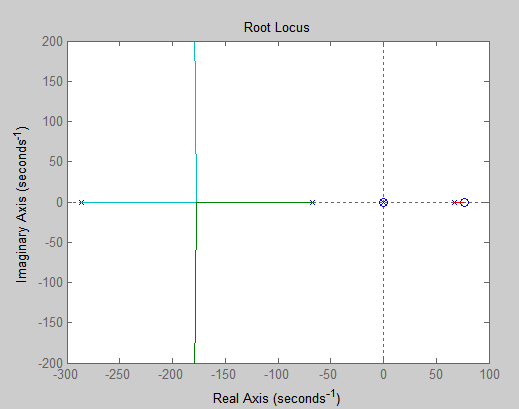
\includegraphics[width=\linewidth]{fig3.PNG}
  \caption{Simulation of system after adding a zero}
  \label{fig:boat1}
\end{figure}
a\subsubsection{Simulation after PI Compensator}
The simulation is shown in Figure 7 on the next page.
\begin{figure}[h]
  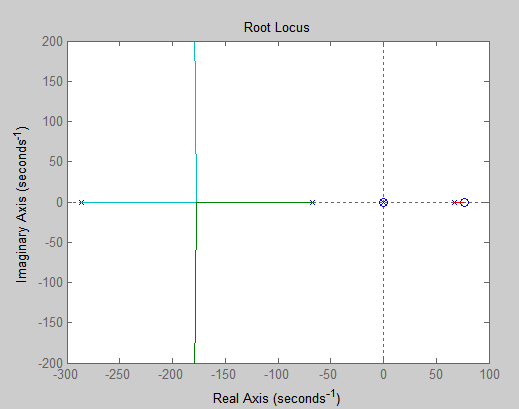
\includegraphics[width=\linewidth]{fig3.PNG}
  \caption{Simulation of system after PI compensator design}
  \label{fig:boat1}
\end{figure}


\end{document}
